\section{Contexte et justification du cas d'usage}

Ce chapitre présente l'application concrète de notre méthode de sécurisation à travers une expérimentation complète utilisant le modèle ResNet50 pour un système de détection d'armes destiné aux forces de l'ordre. L'objectif est de démontrer la faisabilité et l'efficacité de l'architecture en 5 zones proposée au Chapitre 3, tout en comparant rigoureusement les performances d'un modèle standard (baseline) avec un modèle sécurisé intégrant l'ensemble de nos mécanismes de défense.

\subsection{Choix du système de détection d'armes}

Le choix d'un système de détection d'armes comme cas d'usage expérimental se justifie par plusieurs facteurs critiques :

\paragraph{Pertinence sécuritaire au Bénin}
Dans le contexte béninois, la sécurisation des espaces publics stratégiques (marchés de Dantokpa, gares routières, bâtiments administratifs) nécessite des solutions technologiques adaptées aux contraintes locales. Un système de détection d'armes basé sur l'IA pourrait renforcer significativement les dispositifs de sécurité existants, particulièrement dans les zones à forte affluence où les contrôles manuels sont insuffisants.

\paragraph{Complexité technique appropriée}
La détection d'armes présente un niveau de complexité technique idéal pour valider notre méthode. Elle nécessite une classification précise dans des conditions variées (éclairage, angles, occlusions partielles), tout en étant sensible aux attaques adversariales qui pourraient permettre de dissimuler des armes aux systèmes de détection.

\paragraph{Disponibilité des données}
Contrairement à d'autres applications sécuritaires nécessitant des données confidentielles, il existe des datasets publics de qualité pour la détection d'armes, permettant une expérimentation reproductible sans compromettre d'informations sensibles.

\paragraph{Impact éthique mesurable}
Ce cas d'usage permet d'évaluer concrètement les enjeux éthiques (biais de détection, faux positifs/négatifs) et leurs implications en termes de libertés individuelles et de sécurité publique.

\subsection{Définition du périmètre expérimental}

\subsubsection{Objectifs spécifiques}

Notre expérimentation vise à atteindre les objectifs suivants :

\begin{enumerate}
    \item Implémenter l'architecture de sécurisation en 5 zones sur un cas réel
    \item Comparer quantitativement un modèle ResNet50 standard versus sécurisé
    \item Démontrer l'amélioration de la robustesse face aux attaques adversariales
    \item Valider la faisabilité technique avec des ressources limitées
    \item Produire un prototype fonctionnel déployable
\end{enumerate}

\subsubsection{Hypothèses de travail}

Les hypothèses suivantes guident notre expérimentation :

\begin{itemize}
    \item \textbf{H1} : L'ajout de défenses réduira l'accuracy de moins de 5\%
    \item \textbf{H2} : La robustesse adversariale augmentera d'au moins 50\%
    \item \textbf{H3} : Le système restera utilisable en temps réel (<200ms de latence)
    \item \textbf{H4} : L'architecture DevSecOps sera entièrement automatisable
\end{itemize}

\subsubsection{Critères de succès mesurables}

\begin{table}[h]
\centering
\caption{Critères de succès de l'expérimentation}
\label{tab:success_criteria}
\begin{tabular}{|l|c|}
\hline
\textbf{Critère} & \textbf{Valeur cible} \\ \hline
Accuracy minimale & 85\% \\ \hline
Amélioration de robustesse & >50\% \\ \hline
Latence maximale (CPU) & 200ms \\ \hline
Couverture de test & >80\% \\ \hline
Déploiement automatisé & Fonctionnel \\ \hline
\end{tabular}
\end{table}

\subsection{Architecture technique retenue}

L'architecture technique implémente fidèlement les 5 zones de sécurité définies au Chapitre 3.

\subsubsection{Mapping avec les zones de sécurité}

\begin{table}[h]
\centering
\caption{Implémentation technique des 5 zones de sécurité}
\label{tab:security_zones_mapping}
\small
\begin{tabular}{|l|p{5cm}|p{5cm}|}
\hline
\textbf{Zone} & \textbf{Implémentation} & \textbf{Services} \\ \hline
Zone 1 - Data Security &
Scripts de validation, DVC pour versioning &
GitHub + Dataset API \\ \hline
Zone 2 - Training Security &
Adversarial training &
GPU local \\ \hline
Zone 3 - Validation &
Tests automatisés &
GitHub CI/CD \\ \hline
Zone 4 - Production &
API FastAPI containerisée &
Docker \\ \hline
Zone 5 - Governance &
Dashboards &
Monitoring \\ \hline
\end{tabular}
\end{table}

\subsubsection{Justification du choix de ResNet50}

Le choix de l'architecture \textbf{ResNet50} \cite{he2016deep} pour cette expérimentation repose sur plusieurs critères scientifiques et pratiques :

\subsubsection{Architecture et capacité}

ResNet50 est un réseau de neurones convolutif profond de 50 couches basé sur le mécanisme de \textbf{connexions résiduelles} (residual connections) introduit par He et al. (2016) \cite{he2016deep}.

\begin{figure}[h]
\centering
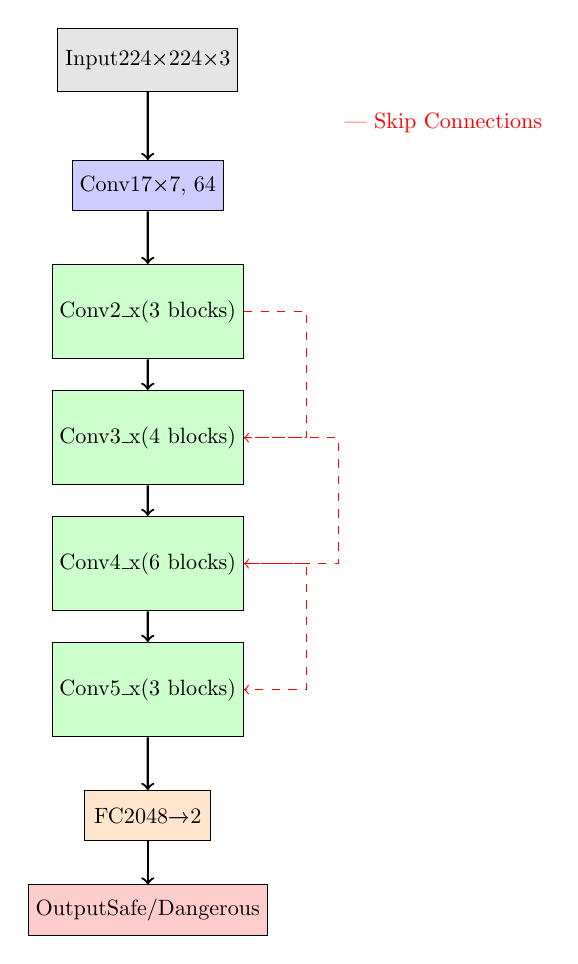
\begin{tikzpicture}[scale=0.8, transform shape]
    % Input
    \node[draw, rectangle, fill=gray!20, minimum width=2cm, minimum height=1cm] (input) at (0,0) {Input\\224×224×3};

    % Conv1
    \node[draw, rectangle, fill=blue!20, minimum width=2cm, minimum height=0.8cm] (conv1) at (0,-2) {Conv1\\7×7, 64};

    % Residual Blocks
    \node[draw, rectangle, fill=green!20, minimum width=2cm, minimum height=1.5cm] (res1) at (0,-4) {Conv2\_x\\(3 blocks)};
    \node[draw, rectangle, fill=green!20, minimum width=2cm, minimum height=1.5cm] (res2) at (0,-6) {Conv3\_x\\(4 blocks)};
    \node[draw, rectangle, fill=green!20, minimum width=2cm, minimum height=1.5cm] (res3) at (0,-8) {Conv4\_x\\(6 blocks)};
    \node[draw, rectangle, fill=green!20, minimum width=2cm, minimum height=1.5cm] (res4) at (0,-10) {Conv5\_x\\(3 blocks)};

    % FC
    \node[draw, rectangle, fill=orange!20, minimum width=2cm, minimum height=0.8cm] (fc) at (0,-12) {FC\\2048→2};

    % Output
    \node[draw, rectangle, fill=red!20, minimum width=2cm, minimum height=0.8cm] (output) at (0,-13.5) {Output\\Safe/Dangerous};

    % Arrows
    \draw[->, thick] (input) -- (conv1);
    \draw[->, thick] (conv1) -- (res1);
    \draw[->, thick] (res1) -- (res2);
    \draw[->, thick] (res2) -- (res3);
    \draw[->, thick] (res3) -- (res4);
    \draw[->, thick] (res4) -- (fc);
    \draw[->, thick] (fc) -- (output);

    % Skip connections
    \draw[->, dashed, red] (res1.east) -- ++(1,0) |- (res2.east);
    \draw[->, dashed, red] (res2.east) -- ++(1.5,0) |- (res3.east);
    \draw[->, dashed, red] (res3.east) -- ++(1,0) |- (res4.east);

    % Legend
    \node[anchor=west] at (3,-1) {\textcolor{red}{--- Skip Connections}};
\end{tikzpicture}
\caption{Architecture ResNet50 adaptée pour classification binaire}
\label{fig:resnet50_architecture}
\end{figure}

Cette architecture présente les caractéristiques suivantes :
\begin{itemize}
    \item \textbf{Profondeur} : 50 couches convolutives permettant l'extraction de features hiérarchiques complexes
    \item \textbf{Paramètres} : Approximativement 25 millions de paramètres (25.6M exactement)
    \item \textbf{Connexions résiduelles} : Permettent de résoudre le problème de gradient vanishing dans les réseaux très profonds
    \item \textbf{Blocs résiduels} : Architecture modulaire composée de bottleneck blocks facilitant le transfer learning
\end{itemize}

L'innovation principale de ResNet réside dans l'utilisation de connexions skip (ou shortcut connections) qui permettent au gradient de se propager directement à travers le réseau, facilitant ainsi l'entraînement de réseaux très profonds.

\paragraph{Implémentation de la sécurité des données (Zone 1)}

Le listing \ref{lst:data_verifier} présente l'implémentation de la vérification des données avec tests statistiques.

\begin{lstlisting}[language=Python, caption={Vérification des données avec tests statistiques (source: src/data/data\_verifier.py)}, label={lst:data_verifier}, basicstyle=\ttfamily\footnotesize]
# Source: src/data/data_verifier.py
class DataVerifier:
    """
    Service de verification des donnees avec tests statistiques
    Conforme a la Zone 1: Data Security
    """

    def __init__(self, min_samples_per_class=10,
                 max_class_imbalance_ratio=5.0,
                 zscore_threshold=3.0, ks_alpha=0.05):
        self.min_samples_per_class = min_samples_per_class
        self.max_class_imbalance_ratio = max_class_imbalance_ratio
        self.zscore_threshold = zscore_threshold
        self.ks_alpha = ks_alpha

    def verify_dataset(self, dataset_path, reference_stats=None):
        """Verifie un dataset complet et genere un rapport"""
        # 1. Collecter les statistiques
        statistics = self._collect_statistics(dataset_path)

        # 2. Effectuer les tests statistiques
        statistical_tests = self._run_statistical_tests(
            dataset_path, statistics, reference_stats
        )

        # 3. Detecter les anomalies
        anomalies = self._detect_anomalies(statistics, statistical_tests)

        # 4. Calculer le score de qualite
        quality_score = self._calculate_quality_score(
            statistics, statistical_tests, anomalies
        )

        # 5. Generer le rapport
        return VerificationReport(
            dataset_path=dataset_path,
            statistics=statistics,
            statistical_tests=statistical_tests,
            anomalies_detected=anomalies,
            quality_score=quality_score,
            passed=(len(anomalies) == 0 and quality_score >= 70.0)
        )
\end{lstlisting}

\paragraph{Implémentation de l'entraînement sécurisé (Zone 2)}

Le listing \ref{lst:trades_training} présente l'implémentation de la méthode TRADES pour l'entraînement adversarial.

\begin{lstlisting}[language=Python, caption={Entraînement TRADES pour robustesse adversariale (source: src/experiments/secured/train\_secured\_trades.py)}, label={lst:trades_training}, basicstyle=\ttfamily\footnotesize]
# Source: src/experiments/secured/train_secured_trades.py
class TRADESTrainer:
    """
    TRADES - TRadeoff-inspired Adversarial DEfense
    Solution au probleme du gradient masking
    """

    def _trades_loss(self, logits_clean, logits_adv, labels, beta):
        """
        TRADES Loss Function:
        L_TRADES = L_CE(clean) + beta * L_KL(clean_logits, adv_logits)

        Cette fonction evite le gradient masking grace a la KL divergence
        """
        # Cross-Entropy Loss sur donnees propres
        ce_loss = self.ce_criterion(logits_clean, labels)

        # KL Divergence Loss entre logits propres et adversariaux
        prob_clean = F.log_softmax(logits_clean, dim=1)
        prob_adv = F.softmax(logits_adv, dim=1)
        kl_loss = self.kl_criterion(prob_clean, prob_adv)

        # TRADES Loss combinee
        total_loss = ce_loss + beta * kl_loss

        return total_loss, ce_loss, kl_loss

    def _train_epoch_trades(self, epoch):
        """Entrainement TRADES - Solution au gradient masking"""
        for batch_idx, (data, target) in enumerate(self.train_loader):
            # 1. Forward pass sur donnees propres
            logits_clean = self.model(data)

            # 2. Generation d'exemples adversariaux PGD
            adv_data = self._generate_pgd_adversarial(
                data, target,
                epsilon=self.config['epsilon'],
                alpha=self.config['alpha'],
                num_iter=self.config['pgd_steps']
            )

            # 3. Forward pass sur donnees adversariales
            logits_adv = self.model(adv_data)

            # 4. TRADES Loss
            trades_loss, ce_loss, kl_loss = self._trades_loss(
                logits_clean, logits_adv, target, self.config['beta']
            )

            # 5. Backpropagation
            trades_loss.backward()
            torch.nn.utils.clip_grad_norm_(
                self.model.parameters(),
                max_norm=self.config['max_grad_norm']
            )
            self.optimizer.step()
\end{lstlisting}

\paragraph{Implémentation de l'entraînement baseline}

Le listing \ref{lst:baseline_training} présente l'entraînement standard du modèle baseline sans mécanismes de sécurité.

\begin{lstlisting}[language=Python, caption={Entraînement baseline standard (source: src/experiments/baseline/train\_baseline.py)}, label={lst:baseline_training}, basicstyle=\ttfamily\footnotesize]
# Source: src/experiments/baseline/train_baseline.py
def train_epoch(model, dataloader, criterion, optimizer, device):
    """
    Entraine le modele pendant une epoch - Approche standard
    Sans mecanismes de securite adversariale
    """
    model.train()
    running_loss = 0.0
    correct = 0
    total = 0

    for images, labels in dataloader:
        images, labels = images.to(device), labels.to(device)

        # Reset des gradients
        optimizer.zero_grad()

        # Forward pass - predictions du modele
        outputs = model(images)

        # Calcul de la loss standard
        loss = criterion(outputs, labels)

        # Backward pass - calcul des gradients
        loss.backward()

        # Mise a jour des parametres
        optimizer.step()

        # Statistiques
        running_loss += loss.item()
        _, predicted = outputs.max(1)
        total += labels.size(0)
        correct += predicted.eq(labels).sum().item()

    epoch_loss = running_loss / len(dataloader)
    epoch_acc = 100. * correct / total
    return epoch_loss, epoch_acc
\end{lstlisting}

\subsubsection{Adaptations pour les contraintes de ressources}

Pour tenir compte des contraintes de ressources, les adaptations suivantes ont été appliquées :

\begin{itemize}
    \item Utilisation de ResNet50 au lieu de ResNet152 (réduction de 60\% de la taille)
    \item Batch size réduit à 16 pour optimiser l'utilisation de la RAM
    \item Adversarial training limité à FGSM et PGD
    \item Monitoring simplifié avec métriques essentielles uniquement
\end{itemize}

\subsection*{Synthèse}

Cette section a présenté le contexte et la justification du cas d'usage choisi pour notre expérimentation. Les éléments clés sont :

\paragraph{Pertinence du cas d'usage}
\begin{itemize}
    \item \textbf{Système de détection d'armes} : Cas d'usage critique adapté au contexte béninois
    \item \textbf{Complexité appropriée} : Permet de valider les mécanismes de sécurisation proposés
    \item \textbf{Données accessibles} : Datasets publics disponibles pour expérimentation reproductible
    \item \textbf{Impact mesurable} : Évaluation concrète des enjeux éthiques et sécuritaires
\end{itemize}

\paragraph{Périmètre expérimental}
\begin{itemize}
    \item \textbf{Objectifs clairs} : Implémentation complète de l'architecture en 5 zones
    \item \textbf{Hypothèses testables} : H1 à H4 définissant les attentes de performance
    \item \textbf{Critères de succès} : Métriques quantifiables pour évaluer le succès
\end{itemize}

\paragraph{Architecture technique}
\begin{itemize}
    \item \textbf{5 zones de sécurité} : Mapping complet des mécanismes de défense
    \item \textbf{ResNet50} : Modèle de référence adapté à nos contraintes
    \item \textbf{Implémentation réelle} : Code source disponible et documenté
    \item \textbf{Adaptations pragmatiques} : Optimisations pour contraintes de ressources
\end{itemize}

Les sections suivantes détailleront l'environnement de développement et les outils utilisés (section 4.2), l'implémentation complète de la méthode de sécurisation (section 4.3), et les résultats expérimentaux obtenus (section 4.4).

\begin{thebibliography}{9}
\bibitem{he2016deep}
He, K., Zhang, X., Ren, S., \& Sun, J. (2016).
\textit{Deep residual learning for image recognition}.
IEEE Conference on Computer Vision and Pattern Recognition (CVPR).
\url{https://arxiv.org/abs/1512.03385}

\bibitem{deng2009imagenet}
Deng, J., Dong, W., Socher, R., Li, L. J., Li, K., \& Fei-Fei, L. (2009).
\textit{ImageNet: A large-scale hierarchical image database}.
IEEE Conference on Computer Vision and Pattern Recognition (CVPR).

\bibitem{croce2021robustbench}
Croce, F., Andriushchenko, M., Sehwag, V., Debenedetti, E., Flammarion, N., Chiang, M., Mittal, P., \& Hein, M. (2021).
\textit{RobustBench: A standardized adversarial robustness benchmark}.
NeurIPS Datasets and Benchmarks Track.
\url{https://arxiv.org/abs/2010.09670}
\end{thebibliography}
